\documentclass[../../spr.tex]{subfiles}

\begin{document}

\section{Testy}
\subsection{Opis metod testowania (np. testy manualne i automatyczne)}

W projekcie zastosowano automatyczne testy integracyjne warstwy kontrolerów w aplikacji Spring Boot.
Testy uruchamiane są na pełnym kontekście aplikacji,
co pozwala na weryfikację poprawności działania endpointów HTTP wraz z rzeczywistą logiką biznesową.
W celu zapewnienia izolacji testów od zewnętrznych systemów, komponenty komunikujące się z
usługami zewnętrznymi są mockowane, natomiast pozostałe serwisy odpowiedzialne za logikę biznesową
działają rzeczywiście. Takie podejście umożliwia sprawdzenie zarówno poprawności odpowiedzi HTTP,
walidacji danych, jak i integracji kontrolerów z warstwą serwisów.
Testy pozwalają na wykrywanie błędów na poziomie integracji, jednocześnie gwarantując stabilność
i powtarzalność testów poprzez eliminację zależności od zewnętrznych systemów.


\subsection{Wyniki testów, napotkane błędy oraz zastosowane rozwiązania}
Przeprowadzone testy integracyjne
potwierdziły poprawność działania endpointów.(\cref{fig:test-results}).
Testy GET na endpointach np. /hall-types, /memberships, /membership-types i /workout-sessions
zwracały kod HTTP 200 oraz listy rekordów, co świadczy o poprawnej implementacji pobierania danych.
Testy POST, takie jak tworzenie nowych sesji treningowych czy członkostw,
zwracały kod HTTP 201, potwierdzając sukces tworzenia rekordów.
Operacje PATCH, np. aktualizacja członkostwa, również działały poprawnie,
zwracając kod 200 i zaktualizowane dane. Testy DELETE, np. usuwanie uczestników
lub ćwiczeń z sesji, kończyły się sukcesem z kodem 204, a następnie weryfikacja GET
potwierdzała usunięcie rekordów. Testy negatywnych scenariuszy,
takich jak pobieranie nieistniejących rekordów czy wysyłanie nieprawidłowych danych,
zwracały odpowiednio kody 404 i 400, co jest zgodne z oczekiwaniami.
Ogólnie, testy wykazały wysoką stabilność API, jeśli byłyby jakieś błędy,
to CI nie wygenerowałby artefaktów, a testy nie przechodziłyby.
\begin{figure}
  \centering
  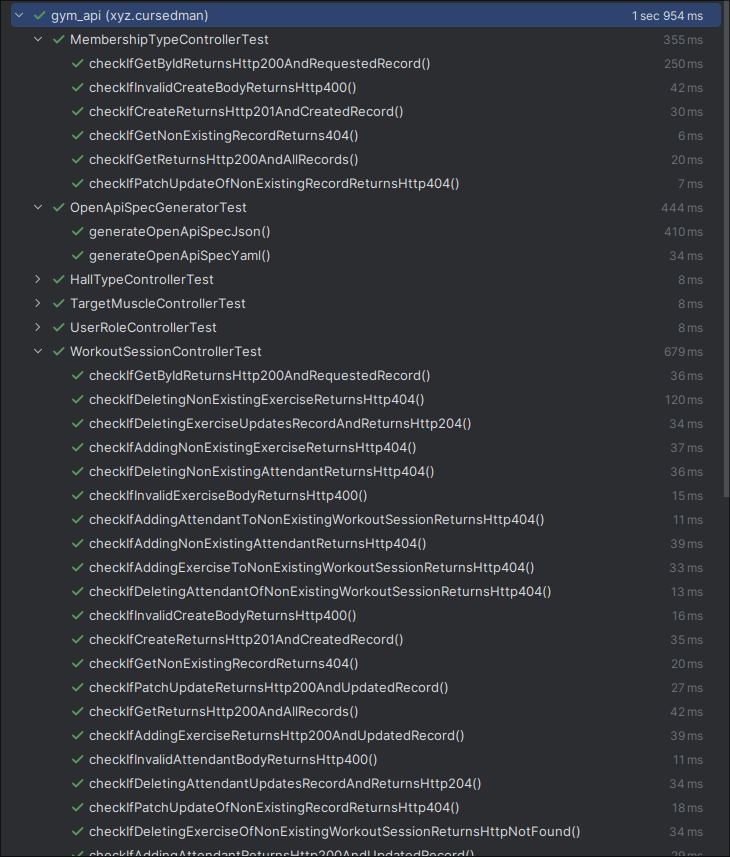
\includegraphics[width=\textwidth]{tests.png}
  \caption{Wyniki testów integracyjnych}
  \label{fig:test-results}
\end{figure}
\end{document}